%\documentclass{sistedes}
\documentclass[12pt]{article}
\usepackage{graphicx}
\begin{document}
\newcommand{\midrule}{\hline}
\newcommand{\toprule}{\hline}
\newcommand{\addlinespace}{\\}
\newcommand{\bottomrule}{\hline}

\title{The depreciation of human capital evidence from Italy }

\author{ Riccardo Dal Cero\inst{1} }

%\institute{ UCSC, Milan, Italy\\
%\email{riccardo.dalcero99@gmail.com}\\
%}

%\maketitle

%\small

%\keywords{Human Capital, Education, Gender gap, ...}

%\publishedin{Journal name, Vol. X, Issue Y, No. Z, pp. xx--yy, YEAR}

\begin{abstract}
This paper seeks to estimate the age-wage profiles and depreciation rates of human capital for different levels of
education in Italy, which are crucial variables that impact overall economic growth and development. To achieve this
goal, we use a dynamic panel dataset provided by the Banks of Italy, covering the period from 1980 to 2019.
\newline
Our analysis aims to estimate the depreciation rates for primary, secondary, and tertiary education levels separately.
By doing so, we provide a comprehensive understanding of the differences in human capital depreciation across various
education levels.
\newline
Furthermore, we also investigate gender differences in human capital depreciation rates. We estimate the depreciation
rates separately for men and women to determine whether there are any differences in the depreciation rates between
genders. This analysis is critical to understanding gender disparities in the labor market, which can have long-term
implications for economic growth and development.
\newline
Overall, our study contributes to the literature on human capital and economic growth by providing insights into the
dynamics of human capital depreciation in Italy. Our findings will be valuable to policymakers and researchers in
designing effective policies to promote economic growth and development in Italy. Additionally, the gender-specific
analysis of human capital depreciation rates will inform policy interventions aimed at promoting gender equality in the
labor market. (Finding) 
% Here, the abstract
\end{abstract}
\newpage
\section{Introduction}
The Ben-Porath model has been widely used in economic research to explain differences in wage-age profiles resulting
from variations in human capital. Human capital encompasses the knowledge, skills, and abilities individuals gain
through education and training, enabling them to participate in the labor market and contribute to the economy. While
human capital is subject to depreciation over time, individuals can invest in their human capital to improve it. The
difference equation that describes human capital includes a depreciation rate, a cohort-specific productivity parameter,
a curvature parameter, and age t.
\newline
Numerous studies have employed the Ben-Porath model to analyze cross-regional differences in wage profiles and the
evolution of wage inequality. However, there is still a need to explore how human capital evolves over time for
individuals with different levels of schooling, with a focus on potential differences in the wage profiles of women.
Understanding the evolution of human capital is crucial to identifying potential constraints to long-term economic
growth, as a population with higher depreciation rates and poor human capital can limit potential growth.
\newline
This paper aims to estimate the age-wage profiles and depreciation rates for different education levels while minimizing
assumptions, following Hendriks' methodology. Additionally, we will examine the impact of gender discrimination on the
long-term human capital of women, which can generate different returns to education. The findings of this study will
provide valuable insights into the dynamics of human capital accumulation and depreciation in Italy. This research also
informs policy interventions aimed at promoting economic growth and development by highlighting potential constraints to
long-term growth and the importance of reducing discrimination in the labor market.
\newline
Ultimately, this research contributes to the broader literature on the role of education and human capital in economic
growth and development, as well as the importance of promoting gender equality in the labor market.

\section{Empirical part}
The empirical questions that we are going to answer are the followings:
\begin{enumerate}
    \item What is the depriciation rate of human capital for different levels of education?
    \item Is there a difference in the depriciation rate between male and female?
\end{enumerate}
\subsection{The model predictions}
The Ben-Porath model suggests that the depreciation rate of human capital is a linear function of time and depends on
the level of human capital. This is because individuals with higher human capital face a higher depreciation rate,
similar to the relationship between capital and growth in the growth theory. As such, we can expect that individuals
with lower education levels, and therefore lower levels of human capital, will experience a lower depreciation rate
compared to those with higher levels of education. \newline
In terms of the wage-age profile, individuals with lower education levels will typically invest less in human capital
and reach their maximum wage sooner and at a lower level compared to those with higher education levels. This is due to
the fact that individuals with higher levels of education are more likely to have specialized skills and knowledge,
which can lead to higher wages and greater career opportunities.
\subsection{Specification}
We use the Conditional Expectation Function (CEF) method to estimate the relationship between the dependent variable:
\begin{itemize}
    \item $log(wage)_{i,y}$
    \item $log(hours)_{i,y}$
\end{itemize}
( and  where $i$ is the individual $i$ of the year $y$) and independent variables:
\begin{itemize}
    \item $age, age^2$: the age and the age squared of the individual $i$ of the year $y$
    \item $i.cohort$ is the list of dummies of the cohorts
    \item $i.years$ is the list of dummies for the years class (class size $=5$).
\end{itemize}
while controlling for:
\begin{itemize}
    \item $educ={3,5}$ Educational level: $3:$ middle school, $5:$ High school level
    \item $sex={0,1}$  Sex $(=1 if female)$
\end{itemize}

There are four specification that we are going to use 
\begin{enumerate}
    \item   \label{spec1}    \(log(wage)_{i,y}=   \beta_1 age_{i}+ \beta_2 age_{i}^2+i.cohort+i.years |educ={3,5}\)
    \item   \label{spec2}    \(log(wage)_{i,y}=   \beta_1 age_{i}+ \beta_2 age_{i}^2+i.cohort+i.years |educ={3,5},sex=
    {0 (male), 1 (female)}\)
    \item   \label{spec3}    \(log(hours)_{i,y}=  \beta_1 age_{i}+ \beta_2 age_{i}^2+i.cohort+i.years |educ={3,5}\)
    \item   \label{spec4}    \(log(hours)_{i,y}= \beta_1 age_{i}+ \beta_2 age_{i}^2+i.cohort+i.years |educ={3,5},sex= {0
    (male), 1 (female)}\)
\end{enumerate}
The CEF method has several limitations. First, it assumes that the age and education variables capture all the relevant
dimensions of human capital, which may not be the case. Other important factors, such as experience or on-the-job
training, are not explicitly considered in the model. Second, the method may suffer from omitted variable bias if there
are unobserved characteristics that affect both wages and education levels. Third, the CEF method assumes that the
relationship between age, education, and wages is linear, which may not hold in reality. Finally, the method relies on
cross-sectional data, which limits the ability to make causal inferences about the effects of education on wages over
time.
\subsection{Identification strategy}
To estimate the depreciation rate of human capital for different levels of education, we need to implement an
identification strategy that allows us to separate the effects of age, education, cohort and year on wage profiles. In
this section, we describe the identification strategy we use in our study.
\newline
To begin with, we assume that the cohort effects are the same for all agents in the same 5-year cohort. This assumption
is motivated by the fact that individuals who are born in the same 5-year period tend to share similar social, economic,
and political experiences during their formative years. For example, individuals who were born during a period of
economic growth may have had more educational opportunities compared to those who were born during a period of economic
recession. By assuming that cohort effects are constant across individuals in the same 5-year cohort, we can control for
unobserved heterogeneity that is specific to a particular cohort.The reasoning behind these assumptions is that in panel
data, we cannot follow the same individual over time due to a lack of a unique identifier. As a result, we cannot
identify individual effects, and we need to impose these restrictions to obtain consistent estimates.
\newline
Secondly, we assume that the initial human endowment is the same within the same cohort. This assumption implies that
individuals who are born in the same 5-year cohort have similar levels of human capital at the beginning of their
careers, before they have invested in additional education or training. By assuming that the initial human endowment is
constant within the same cohort, we can control for unobserved heterogeneity that is specific to a particular birth
cohort.
\newline
The same assumption applies to year effects, meaning that individuals within the same cohort experience the same effects
on wages over a period of 5 years.
\newline
The restrictions imposed on the model are based on some naive assumptions about the behavior of individuals with respect
to their education and human capital. For instance, it is reasonable to assume that individuals who are born in the same
5-year cohort would have similar opportunities for education and training. Similarly, individuals who start with the
same initial human capital endowment within the same cohort are likely to face similar labor market opportunities over
time.\newline
While these assumptions may not hold perfectly in reality, they provide a useful framework for identifying the key
factors that drive the age-wage profile and depreciation rates of human capital for different levels of education in
Italy. By controlling for cohort and year effects in our analysis, we can isolate the effect of age and education on
wages and estimate the rate of human capital depreciation for different groups of individuals.
\newline
To estimate the depreciation rate of human capital for different levels of education, we use a dynamic panel data
approach. Specifically, to estimate the age-wage profiles and the depreciation rates of human capital for different
levels of education in Italy, we employ an OLS approach. We run two separate OLS regressions for individuals with a
lower-secondary education and those with a high school level education, respectively. The dependent variable is the
natural logarithm of the wage, and the key independent variables are age and age squared. We control for cohort effects
and year effects by including birth year dummies and calendar year dummies, respectively. Additionally, the wage
variable is corrected for inflation using the consumer price index.
\newline
Moreover, to examine gender differences in the evolution of human capital, we perform four separate regressions
conditioned on gender and two levels of education, as specified in\ref{spec2}. To capture the potential variation in
gender effects over time, we employ the regression on the conditional expectation function. Additionally, we use the
same methodology to estimate the gender gap in the hours-age profile.
\newline
 Applied Overall, our identification strategy allows us to separate the effects of age, education, and cohort on wage
 profiles and estimate the depreciation rate of human capital for different levels of education. By using a dynamic
 panel data approach and controlling for individual-specific unobserved heterogeneity and time-varying factors, we can
 obtain more accurate estimates of the depreciation rate of human capital, which is a crucial variable that affects
 overall economic growth and development.
\section{Data and descriptive statistics}
\subsection{Data}
The data used in this study are obtained from the Family Income Survey of the Bank of Italy, which spans a period from
1980 to 2020 with $\sim100.000 obs$. The sample comprises both men and women born between 1940 and 2020. To expand our
sample size, we have divided the population into 56 birth cohorts, where each cohort covers five consecutive birth
years. We have also applied the same division for years, where each group includes five years. The following table
\ref{desc-cohort} tabulate the distribution on observations for cohort. The cohort with the highest density of
observations is cohort 10, whereas the younger and older cohorts have relatively few observations. The objective of the
study is to estimate wage-age profiles, which required the use of employee income reports merged with family and
individual statistics. To calculate $\log(wagei,t)$, we employed a series of transformations. Firstly, we summed the
monetary and non-monetary components of income. Secondly, we deflated the income figures using the Consumer Price Index
(CPI). Thirdly, we divided the income figures by the monthly hours worked and multiplied by 13 months to obtain the
annual income. Fourthly, we took the logarithm of the annual income figure. Finally, we merged the resulting dataset
with individual-level data.
\newline
The process of computing \(\log(wage_{i,t})\) was essential for the analysis, as it allowed us to measure the variation
in wages over time, which is critical for estimating wage-age profiles. By merging different datasets, we were able to
obtain a more comprehensive picture of the factors influencing wage dynamics in Italy. We follow these steps to get
\(\log(wage_{i,t})\):
\begin{enumerate}
    \item Sum monetary and non monetary components 
    \item Deflating for CPI
    \item dividing for the mountly hours and multiply for 13 month
    \item take logs
    \item merging with other dataset with individual data
\end{enumerate}
\subsection{Descriptive statistics}

The tables presented in this paper (see Tables\ref{desc-table1a} and\ref{desc-table1b}) display the mean, standard
error, and t-test for difference in mean for log(wage) and annual working hours for four different groups based on
education level and gender: those with a low level of secondary school education, those with a secondary school
education level, and these subgroups further differentiated by sex. The statistical results suggest that individuals
with a secondary school education level tend to earn higher wages than those with a lower level of education. However,
the wage gap between genders is more pronounced among those with a secondary school education level. In other words,
women tend to earn less than men across all education levels, and the difference is wider for those with a higher level
of education.
\newline
In terms of annual working hours, the statistics indicate that individuals with a lower level of education tend to work
more hours than those with a higher level of education. However, this trend is reversed when looking at gender
differences. Women tend to work fewer hours compared to men across all education levels. Interestingly, this gender gap
in working hours narrows as the level of education increases. It is important to note that the data used in the analysis
covers a period from 1980 to 2020, during which the participation of women in the labor market has increased
significantly. Thus, the true difference in working hours between genders may be even greater for individuals with the
same characteristics.\newline
In order to better understand the relationship between education level and economic outcomes, it is often useful to
examine a specific cohort in a given year. This approach is particularly relevant when working with panel data, as it
allows for a more detailed analysis of trends and patterns over time. By focusing on a single cohort, we can examine the
distribution of key economic variables such as wage, income, and annual hours worked, conditional on different levels of
education. This type of analysis can reveal important insights into the labour market for specific subgroups, and help
to identify disparities and trends that may not be apparent when analysing data at the aggregate level.
\newline
The table\ref{desc-cohort} presented in this study reports on the wage and working hours of a specific cohort in the
year 2008. The descriptive statistics show that wages are positively correlated with education level, which is
consistent with the trend observed in the previous  tables\ref{desc-table1a}\ref{desc-table1b}. Additionally, the
statistics reveal a decreasing trend in working hours as the level of education increases. This finding suggests that
individuals with higher levels of education are able to earn higher wages while working fewer hours, potentially due to
their possession of skills or abilities that increase their productivity as according to the human capital model. It is
important to note that this specific cohort has a mean age of 50, which is a significant age for the human capital
model. This is because at this age, individuals have typically spent their time endowments in work without investing in
human capital. Therefore, these summary statistics must be interpreted in light of the fact that this cohort represents
middle-aged workers who have already invested significant time and resources into their careers.\newline
In conclusion, the descriptive statistics presented in this paper provide valuable insights into the labor market
outcomes of individuals with different levels of education. Our analysis revealed that, on average, individuals with
higher levels of education tend to earn higher wages and work fewer hours than those with lower levels of education. We
also found that there are significant gender disparities in labor market outcomes, with women generally earning less and
working fewer hours than men.
\section{Empirical results}
This section presents our findings on the difference in the human capital evolution for different education and gender
characteristics. First, we examine whether attain secondary education level change the wage age profile. Furthermore if
there exists some gender differences in the wage age profile for the same level of education. Second, we focus in
estimating the hours-age profile for the same subgroups.
\subsection{The estimation of wage age profile}
According to the human capital theory, the wage-age profile reflects the relationship between an individual's age and their wages, which is influenced by their investment in human capital over time. To explore this relationship, we use regression analysis with specification\ref{spec1} and present the results in Table \ref{reg1}. The key parameters include $\beta_{age2}$, which indicates the decline in wages over time and reflects depreciation, and $\beta_{age}$, which represents the return on investment in human capital over time. All the coefficients are statistically significant, providing valuable insights into the dynamics of the labor market and the role of human capital investments in shaping the wage-age profile.

If we focus on individuals with lower education\ref{reg1b}, the results indicate that an increase of one year in age leads to an increase of approximately 10.3\% in wages. On the other hand, for individuals with higher education \ref{reg1b}, an increase of one year in age leads to an increase of approximately 12.2\% in wages. These findings are consistent with the human capital theory, which suggests that having a secondary level education instead of a lower secondary education leads to higher returns, while the depreciation rate remains the same for both groups. The low value of $\bar{R}^2$ suggests that the regression has limited predictive power, possibly due to the restrictions imposed to isolate the cohort and year fixed effects.
\newline
To visually inspects the results we show the predicted
wages by cohorts.
\newline
The graph\ref{fig:pred_reg} provides a visual representation of the relationship between education levels and wages across different age cohorts. The findings support the theory that higher levels of human capital lead to higher wages. Specifically, the graph shows that individuals with higher education levels consistently earn higher wages compared to those with lower education levels across all age cohorts.
\newline
Furthermore, the graph also shows that the wage gap between education levels widens over time. This suggests that younger cohorts have a smaller wage gap because the lower-educated individuals are more experienced in the labor market, while the higher-educated individuals are just starting out. However, as time goes by, the market starts to remunerate better those individuals who have invested in higher human capital.
\newline
Building upon these findings, we extend our analysis to include the effects of gender on wages by conducting a regression analysis similar to the one before but with gender as a conditioning variable. This will allow us to examine the gender wage gap across different education levels and age cohorts, providing important insights into the dynamics of the labor market and the role of gender in wage determination.
\newline
The table \ref{reg2} shows clear evidence of a lower return on education for females, with $\beta_{2,female}$ being less than $\beta_{2,male}$. This gap is even wider for individuals with higher levels of education, as $\Delta_{secondary}$ is less than $\Delta_{lower\ secondary}$. 
The gender gap in wages can be decomposed into two factors that widen it over time: firstly, the increase in wages as a result of acquiring working experience represented by $\beta_{Age}$, and secondly, the decrease in wages represented by $\beta_{Age^2}$.

Further analysis reveals that women have lower remuneration for human capital, as seen in the results in columns (3) and (4) of table \ref{reg2}. For the same level of education, the remuneration increases slightly over the years, but by approximately 3\% less for women compared to men. This finding justifies the wide difference in wages shown in table\ref{desc-table1a}. 
The regression results in columns (1)\ref{2.a_m_s}, (2)\ref{2.a_m_ls}, and (3)\ref{2.a_f_s} indicate that there is no significant difference in the depreciation rate between genders. However, in column (4)\ref{2.a_f_ls}, a lower depreciation rate is observed for females with higher levels of education, suggesting that the negative difference in depreciation rates is wider for females with higher education compared to males. \newline
The results highlight the importance of considering gender as a conditioning variable in wage regression analysis, as it provides valuable insights into the dynamics of the labor market and the role of human capital investments in shaping the wage-age profile.
To better understand the difference in the evolution of wage-age
profiles for women and men, we plot a chart of the predicted $\log(wage)$ comparing individuals with the same level of education but with different
gender.
\newline
The chart\ref{fig:w_gend_l} illustrates that male wage-age profiles do not differ widely than women across all cohorts. 
Now we take a look at the same results for secondary school. 
\newline
The chart in Figure\ref{fig:w_gend_h} illustrates a lower gender gap in wage-age profiles compared to the previous chart\ref{fig:w_gend_l}. 
\newline
Overall the estimate return in education are consistent with the human capital theory even here the comparison was by
individual with lower secondary and secondary education level, it would had been better the comparison with individuals
with a bachelor. However it is not possible since the are only few observations $\approx 600$ to get significant estimate
of the key dependent variables.

\subsection{The estimation of hour age profile}
Working hours is a fundamental variable in the human capital model, as it is the outcome of an optimization process
whereby individuals choose how much of their time endowment to allocate towards increasing their human capital, and how
much to devote to working. In this sense, working hours can be seen as a proxy for investment in human capital, as
individuals who invest more time in developing their skills and knowledge may have fewer hours available for paid
work.\newline
First, we will look at difference in the hours- age profiles for individual with different levels of education. Second we
will look at difference in the hours-age profile as before but conditioning on gender. In the following table\ref{reg3}, we estimate with OLS the second specification\ref{spec2} for lower secondary and secondary education level.
\newline
In Table\ref{reg3}, our analysis shows that individuals with lower levels of education tend to start working earlier in life, compared to those with higher education. This is reflected in the negative coefficients of the Age variable in column (2), indicating that annual working hours tend to decrease over time for this group. 
\newline
On the other hand, for those who spend more time in school, the slope of the hours-age relationship is positive, which is consistent with the idea that higher-educated individuals tend to increase the number of hours worked over time, as they continue to invest in their human capital early in their careers, and gradually reduce their working hours as they gain experience. 
Indeed,The Human capital model predicts that individuals with lower education levels tend to start working earlier in life to maximize their immediate earnings, while those with higher education may delay their entry into the labor market as they invest in their human capital.
\newline
To visually inspect these results, we plot the predicted values for working hours by education level, separating each
cohort (figure.\ref{fig:hours}). This allows us to see the trends in working hours across different levels of education for each cohort,
providing further insight into the relationship between human capital and working hours
\newline
In the presented graph, the red line represents the hours-age profiles for individuals with lower secondary school education. These individuals tend to start spending their time endowment working earlier compared to those with secondary education. Additionally, individuals with lower education have a higher hours-age profile, which decreases over time. 
The peak of the red group's hours-age profile is reached in the early years of their working career, and then the curve slightly decreases over time. In contrast, for those with higher education, the peak is reached between 40 and 50 years old, and then starts to decrease. 
It is important to emphasize that individuals with higher education spend less time working for all years, and this trend is observed in all cohorts.
\newline
To look a gender differences in the hours-age profile we run the same regression specification as above\ref{spec4}, but conditioning on gender. The results are showed in the table\ref{reg4}. As in the results without conditioning on gender, the slope of the hours-age profile is negative for individual with higher education level. Notwithstanding, for women the slope are flatter across all level of education, meaning that women increases more mildly the time spent working.
Moreover, female with low education has a steeper negative hours-age profiles, signaling that low educated women tends to decrease at faster rate the participation in the labour market in the intensive margin.  
\newline
To visually compare the predicted working hours by cohort for males (in red) and females (in blue) at different levels of education, we plotted the results in Figure\ref{fig:h_l_cohorts} and Figure\ref{fig:h_h_cohorts}. The hours-age profiles for lower educated women were consistently lower than for men across all cohorts, indicating that this gender gap persists over time. However, for higher educated individuals, the gender differences were not apparent (as shown in Figure \ref{fig:h_h_cohorts}).
\newline
Overall, our empirical findings are in line with the human capital theory, as we found a positive and statistically significant effect of education on human capital remuneration, and a concave wage-age profile as predicted by the model with depreciation $\Delta > 0$. Additionally, the hours-age profile supports the human capital model's predictions, with higher educated individuals having an increasing hours-age profile, and lower educated individuals having a decreasing one.
\section{Conclusions}
In conclusion, this paper has provided an analysis of the gender wage gap in a European country, focusing on the role of education and human capital. The empirical findings are consistent with the human capital theory, as we observe a positive statistically significant effect of education on the remuneration of human capital and a concave shape of the wage-age profile, in line with the model with $\Delta > 0$.
\newline
Furthermore, the analysis shows that the gender wage gap widens over time, mainly due to differences in the remuneration of human capital between men and women. Women have a lower remuneration of human capital, even for the same level of education, which can be partly explained by differences in working hours, as women tend to invest less time in developing their skills and knowledge.
\newline
The results also indicate that individuals with lower levels of education start working earlier, with the aim of maximizing their immediate earnings, while those with higher levels of education may take longer to start working as they invest in their human capital. This is reflected in the hours-age profile, which decreases over time for those with lower education, while it increases for those with higher education.
\newline
However, it is important to note that the analysis has certain limitations. Firstly, the restriction imposed on cohort fixed effects and years fixed effects, which may not capture all the heterogeneity in the data. Secondly, the analysis only focuses on a single country, and the results may not be generalizable to other contexts. Finally, the study does not account for the potential impact of discrimination and other factors that may contribute to the gender wage gap.
\newline
Overall, this study provides insights into the factors that contribute to the gender wage gap and highlights the importance of education and human capital in determining individuals' earnings. Further research is needed to explore the role of other factors, such as discrimination and family responsibilities, and to investigate the effectiveness of policies aimed at reducing the gender wage gap.






\newpage
\section{Tables}
\begin{center}
    \begin{table}[htbp]\centering
    \def\sym#1{\ifmmode^{#1}\else\(^{#1}\)\fi}
    \caption{\label{Tab:desc-1a}Descriptive statistics wages}
    \begin{tabular}{l*{4}{c}}
        \hline

        \multicolumn{1}{c}{Education level}   &\multicolumn{1}{c}{Male}&\multicolumn{1}{c}{Female}&\multicolumn{1}{c}{Diff.}\\
                        \\
        \hline
        Lower Secondary &       51.71           &    48.06          &   3.642061\sym{***} \\
                        &       (33.06)         &   (40.60)         &  (.9713213)       \\
        Secondary       &       124.03          &    113.09         &   5.360341\sym{***}   \\
                        &       (91.37)         &   (73.14)         &   (.5809988 )       \\
        Diff.           &       -18.47816\sym{***} &   -16.75988\sym{***} &                      \\
                        &       (.7922257)  &   (1.07596)           &                       \\
        \\
        \hline
        \multicolumn{3}{l}{\footnotesize Standard errors in parentheses}\\
        \multicolumn{3}{l}{\footnotesize }\\
        \multicolumn{3}{l}{\footnotesize \sym{*} \(p<0.10\), \sym{**} \(p<0.05\), \sym{***} \(p<0.01\)}\\

    \end{tabular}
\end{table}
\begin{table}[htbp]\centering
    \def\sym#1{\ifmmode^{#1}\else\(^{#1}\)\fi}
    \caption{\label{Tab:desc-1b}Descriptive statistics annual working hours}
    \begin{tabular}{l*{4}{c}}
        \hline
        \multicolumn{1}{c}{Education level}   &\multicolumn{1}{c}{Male}&\multicolumn{1}{c}{Female}&\multicolumn{1}{c}{Diff}\\
        \\
        \hline
            Lower Secondary & 1,952.12      & 1,642.11& 310.0051\sym{***}  \\
                            & (393.85)      & (537.70)& (12.13044)  \\
            Secondary       &  1,811.48     & 1,507.51& 253.783\sym{***}      \\
                            & (484.11)      & (491.03)& (4.887414)    \\
            Diff.           &       27.01869 \sym{***}   & -29.20347\sym{***}\\
                            &       (6.180364)  &   (11.81991)  \\
        \\                    
        \hline
        \multicolumn{3}{l}{\footnotesize Standard errors in parentheses}\\
        \multicolumn{3}{l}{\footnotesize }\\
        \multicolumn{3}{l}{\footnotesize \sym{*} \(p<0.10\), \sym{**} \(p<0.05\), \sym{***} \(p<0.01\)}\\


    \end{tabular}
\end{table}

    \begin{tabular}{l*{6}{c}}
\toprule
                &   no edu&  primary&lower secondary&secondary technical - 3 years&secondary&first level degree\\
\midrule
Mean of log(wage)&     3.61&     3.63&     3.67&     3.69&     3.75&     3.66\\
                &      (.)&   (0.06)&   (0.03)&   (0.02)&   (0.02)&   (0.06)\\
\addlinespace
Mean of work hour& 1,920.00& 1,886.70& 1,811.86& 1,780.06& 1,678.31& 1,828.11\\
                &      (.)& (116.59)&  (50.03)&  (31.46)&  (38.77)& (116.77)\\
\addlinespace
mean\_y          & 71261.03& 71261.03& 71261.03& 71261.03& 71261.03& 71261.03\\
                &      (.)&   (0.00)&   (0.00)&   (0.00)&   (0.00)&   (0.00)\\
\addlinespace
Sex             &     0.00&     0.26&     0.40&     0.55&     0.66&     0.57\\
                &      (.)&   (0.45)&   (0.49)&   (0.50)&   (0.48)&   (0.53)\\
\bottomrule
\end{tabular}

    {
\def\sym#1{\ifmmode^{#1}\else\(^{#1}\)\fi}
\begin{tabular}{l*{5}{c}}
\hline
            &\multicolumn{1}{c}{(Cohort)} & \multicolumn{1}{c}{N.obs} & & \multicolumn{1}{c}{Freq.}& \multicolumn{1}{c}{Perc.} & \multicolumn{1}{c}{Cum.}\\
\hline
1           &          42         & 0.04      &  0.04\\
            &                     \\

2           &         619    &0.59     &   0.63       \\
            &                     \\

3           &        1816    & 1.74     &   2.37    \\
            &                     \\

4           &        3333   & 3.20   &     5.57     \\
            &                     \\

5           &        6869    &6.58     &  12.15     \\
            &                     \\

6           &        9495    &9.10   &    21.26     \\
            &                     \\

7           &       11401     &10.93   &    32.19    \\
            &                     \\

8           &       11971    &11.48      & 43.66     \\
            &                     \\

9           &       13347    &12.79     &  56.46     \\
            &                     \\

10          &       14240    & 13.65  &     70.11    \\
            &                     \\

11          &       10862  & 10.41   &    80.52      \\
            &                     \\

12          &        8222    &7.88    &   88.40     \\
            &                     \\

13          &        6291  &6.03  &     94.43       \\
            &                     \\

14          &        4291  &  4.11  &     98.55     \\
            &                     \\

15          &        1517   & 1.45 &     100.00      \\
            &                     \\
\hline
Total       &      104316         \\
            &                     \\

\multicolumn{2}{l}{\footnotesize \textit{t} statistics in parentheses}\\
\multicolumn{2}{l}{\footnotesize \sym{*} \(p<0.05\), \sym{**} \(p<0.01\), \sym{***} \(p<0.001\)}\\
\end{tabular}
}

    \begin{table}[htbp]\centering
\def\sym#1{\ifmmode^{#1}\else\(^{#1}\)\fi}
\caption{Regression table \label{reg1}}
\begin{tabular}{l*{2}{c}}
\toprule
                    &\multicolumn{1}{c}{(1)}         &\multicolumn{1}{c}{(2)}         \\
\midrule
Age                 &       0.126\sym{***}&       0.109\sym{***}\\
                    &     (0.018)         &     (0.006)         \\
                    \\
                    Cohort f.e           &       Yes        &      Yes \\
                                                \\
                    \addlinespace
                    years f.e.            &       Yes         &       Yes         \\
                                               \\
                    \addlinespace
Constant            &      -0.199         &       0.038         \\
                    &     (0.784)         &     (0.475)         \\
\midrule
Observations        &       10088         &       28968         \\
\bottomrule
\multicolumn{3}{l}{\footnotesize Standard errors in parentheses}\\
\multicolumn{3}{l}{\footnotesize }\\
\multicolumn{3}{l}{\footnotesize \sym{*} \(p<0.10\), \sym{**} \(p<0.05\), \sym{***} \(p<0.01\)}\\
\end{tabular}
\end{table}

    \begin{table}[htbp]\centering
    \def\sym#1{\ifmmode^{#1}\else\(^{#1}\)\fi}
    \caption{Regression table \label{reg2}}
    \begin{tabular}{l*{4}{c}}
    \hline
                        &\multicolumn{1}{c}{(1) M. L.Sec.}\label{2.a_m_ls}         &\multicolumn{1}{c}{(2) M.
                        Sec.}\label{2.a_m_s}        &\multicolumn{1}{c}{(3)F. L.Sec.}\label{2.a_f_ls}        &\multicolumn{1}{c}{(4)F.
                        Sec}\label{2.a_f_s}
                        \\
    \hline
    Age                 &     0.13526\sym{***}&     0.11087\sym{***}&     0.10669\sym{***}&     0.09855\sym{***}\\
                        &   (0.03060)         &   (0.01950)         &   (0.00757)         &   (0.00999)         \\
    \\
    age2                &    -0.00087\sym{***}&    -0.00081\sym{***}&    -0.00087\sym{***}&    -0.00068\sym{***}\\
                        &   (0.00032)         &   (0.00021)         &   (0.00008)         &   (0.00010)         \\
    \\
    Cohort fixed effect           &       Yes        &       Yes      & Yes & Yes  \\
    Years (5 year class) fixed effect             &       Yes       &       Yes      & Yes  & Yes   \\
    \hline
    Observations        &        4669         &        5626         &       19337         &       10114         \\
    \hline
    \multicolumn{5}{l}{\footnotesize Standard errors in parentheses}\\
    \multicolumn{5}{l}{\footnotesize }\\
    \multicolumn{5}{l}{\footnotesize \sym{*} \(p<0.10\), \sym{**} \(p<0.05\), \sym{***} \(p<0.01\)}\\
    \end{tabular}
    \end{table}
    
    \begin{table}[htbp]\centering
\def\sym#1{\ifmmode^{#1}\else\(^{#1}\)\fi}
\caption{Regression \(E[log(Hours)|educ]\) \label{Tab:reg3}}
\begin{tabular}{l*{2}{c}}
\toprule
                    &\multicolumn{1}{c}{(1)\(educ=1\)\label{Reg:3_h}}         &\multicolumn{1}{c}{\(educ=0\)\label{Reg:3_l}}         \\
\midrule
Age                 &       0.031\sym{***}&      -0.007\sym{***}\\
                    &     (0.003)         &     (0.000)         \\
\addlinespace
age2                &      -0.000\sym{***}&       0.000\sym{***}\\
                    &     (0.000)         &     (0.000)         \\
\addlinespace
age2                &      -0.000\sym{*}  &       0.000         \\
                    &     (0.000)         &     (0.000)         \\
\\
Cohort f.e           &       Yes        &      Yes \\
                            \\
\addlinespace
years f.e.            &       Yes         &       Yes         \\
                           \\
\addlinespace
Constant            &       6.786\sym{***}&       7.833\sym{***}\\
                    &     (0.166)         &     (0.020)         \\
\midrule
Observations        &       10088         &       28968         \\
$R^2$ overall       &   0.0345&0.3897 \\
\bottomrule
\multicolumn{3}{l}{\footnotesize Standard errors in parentheses}\\
\multicolumn{3}{l}{\footnotesize }\\
\multicolumn{3}{l}{\footnotesize \sym{*} \(p<0.10\), \sym{**} \(p<0.05\), \sym{***} \(p<0.01\)}\\
\end{tabular}
\end{table}

    \begin{table}[htbp]\centering
\def\sym#1{\ifmmode^{#1}\else\(^{#1}\)\fi}
\caption{Regression table \label{reg4}}
\begin{tabular}{l*{4}{c}}
\toprule
                    &\multicolumn{1}{c}{(1)}         &\multicolumn{1}{c}{(2)}         &\multicolumn{1}{c}{(3)}         &\multicolumn{1}{c}{(4)}         \\
\midrule
Age                 &     0.00664\sym{***}&     0.00428\sym{***}&    -0.00655\sym{***}&    -0.00689\sym{***}\\
                    &   (0.00084)         &   (0.00073)         &   (0.00024)         &   (0.00034)         \\
\addlinespace
age2                &    -0.00006\sym{***}&    -0.00003\sym{***}&     0.00003\sym{***}&     0.00004\sym{***}\\
                    &   (0.00001)         &   (0.00001)         &   (0.00000)         &   (0.00000)         \\
\addlinespace
Cohort=1            &     0.00000         &     0.00000         &     0.00000         &     0.00000         \\
                    &         (.)         &         (.)         &         (.)         &         (.)         \\
\addlinespace
Cohort=2            &    -0.10875\sym{***}&    -0.10144\sym{**} &     0.02052         &    -0.00604         \\
                    &   (0.02585)         &   (0.04229)         &   (0.01927)         &   (0.05698)         \\
\addlinespace
Cohort=3            &    -0.03457         &    -0.04720         &    -0.01953         &    -0.02148         \\
                    &   (0.02497)         &   (0.04103)         &   (0.01895)         &   (0.05504)         \\
\addlinespace
Cohort=4            &    -0.13421\sym{***}&    -0.13423\sym{***}&    -0.03231\sym{*}  &    -0.02966         \\
                    &   (0.02515)         &   (0.04082)         &   (0.01892)         &   (0.05493)         \\
\addlinespace
Cohort=5            &    -0.12895\sym{***}&    -0.10977\sym{***}&    -0.06005\sym{***}&    -0.05568         \\
                    &   (0.02558)         &   (0.04094)         &   (0.01898)         &   (0.05494)         \\
\addlinespace
Cohort=6            &    -0.10098\sym{***}&    -0.08635\sym{**} &    -0.08488\sym{***}&    -0.07619         \\
                    &   (0.02629)         &   (0.04125)         &   (0.01910)         &   (0.05501)         \\
\addlinespace
Cohort=7            &    -0.10419\sym{***}&    -0.08325\sym{**} &    -0.09141\sym{***}&    -0.07899         \\
                    &   (0.02712)         &   (0.04169)         &   (0.01927)         &   (0.05512)         \\
\addlinespace
Cohort=8            &    -0.07086\sym{**} &    -0.04956         &    -0.11222\sym{***}&    -0.09736\sym{*}  \\
                    &   (0.02813)         &   (0.04224)         &   (0.01947)         &   (0.05526)         \\
\addlinespace
Cohort=9            &    -0.05504\sym{*}  &    -0.04042         &    -0.13059\sym{***}&    -0.11586\sym{**} \\
                    &   (0.02922)         &   (0.04282)         &   (0.01969)         &   (0.05542)         \\
\addlinespace
Cohort=10           &    -0.03127         &    -0.01890         &    -0.15453\sym{***}&    -0.13872\sym{**} \\
                    &   (0.03048)         &   (0.04347)         &   (0.01995)         &   (0.05560)         \\
\addlinespace
Cohort=11           &    -0.05609\sym{*}  &    -0.02720         &    -0.16540\sym{***}&    -0.14791\sym{***}\\
                    &   (0.03172)         &   (0.04420)         &   (0.02021)         &   (0.05579)         \\
\addlinespace
Cohort=12           &    -0.04494         &    -0.01918         &    -0.20371\sym{***}&    -0.18665\sym{***}\\
                    &   (0.03305)         &   (0.04493)         &   (0.02052)         &   (0.05601)         \\
\addlinespace
Cohort=13           &    -0.05757\sym{*}  &    -0.03701         &    -0.22877\sym{***}&    -0.20986\sym{***}\\
                    &   (0.03451)         &   (0.04579)         &   (0.02087)         &   (0.05627)         \\
\addlinespace
Cohort=14           &    -0.01332         &    -0.00896         &    -0.28138\sym{***}&    -0.26166\sym{***}\\
                    &   (0.03634)         &   (0.04685)         &   (0.02121)         &   (0.05651)         \\
\addlinespace
years=1             &     0.00000         &     0.00000         &     0.00000         &     0.00000         \\
                    &         (.)         &         (.)         &         (.)         &         (.)         \\
\addlinespace
years=2             &     0.01534\sym{***}&     0.00525         &    -0.00064         &    -0.00326\sym{*}  \\
                    &   (0.00355)         &   (0.00335)         &   (0.00126)         &   (0.00180)         \\
\addlinespace
years=3             &     0.04231\sym{***}&     0.03728\sym{***}&     0.00662\sym{***}&     0.00285         \\
                    &   (0.00488)         &   (0.00444)         &   (0.00178)         &   (0.00255)         \\
\addlinespace
years=4             &     0.03696\sym{***}&     0.02753\sym{***}&     0.02034\sym{***}&     0.01552\sym{***}\\
                    &   (0.00657)         &   (0.00594)         &   (0.00243)         &   (0.00345)         \\
\addlinespace
years=5             &     0.02608\sym{***}&     0.01363\sym{*}  &     0.02264\sym{***}&     0.02156\sym{***}\\
                    &   (0.00858)         &   (0.00770)         &   (0.00322)         &   (0.00452)         \\
\addlinespace
years=6             &     0.01209         &     0.00031         &    -0.00049         &    -0.01338\sym{**} \\
                    &   (0.01015)         &   (0.00901)         &   (0.00382)         &   (0.00539)         \\
\addlinespace
Cohort=15           &                     &                     &    -0.06478\sym{***}&    -0.05879         \\
                    &                     &                     &   (0.02161)         &   (0.05680)         \\
\addlinespace
Constant            &     7.30019\sym{***}&     7.32478\sym{***}&     7.83727\sym{***}&     7.82594\sym{***}\\
                    &   (0.03770)         &   (0.04731)         &   (0.02118)         &   (0.05648)         \\
\midrule
Observations        &        5293         &        6370         &       26561         &       16663         \\
\bottomrule
\multicolumn{5}{l}{\footnotesize Standard errors in parentheses}\\
\multicolumn{5}{l}{\footnotesize }\\
\multicolumn{5}{l}{\footnotesize \sym{*} \(p<0.10\), \sym{**} \(p<0.05\), \sym{***} \(p<0.01\)}\\
\end{tabular}
\end{table}

\end{center}
\newpage

\section{Figures}

\begin{figure}
    \centering
    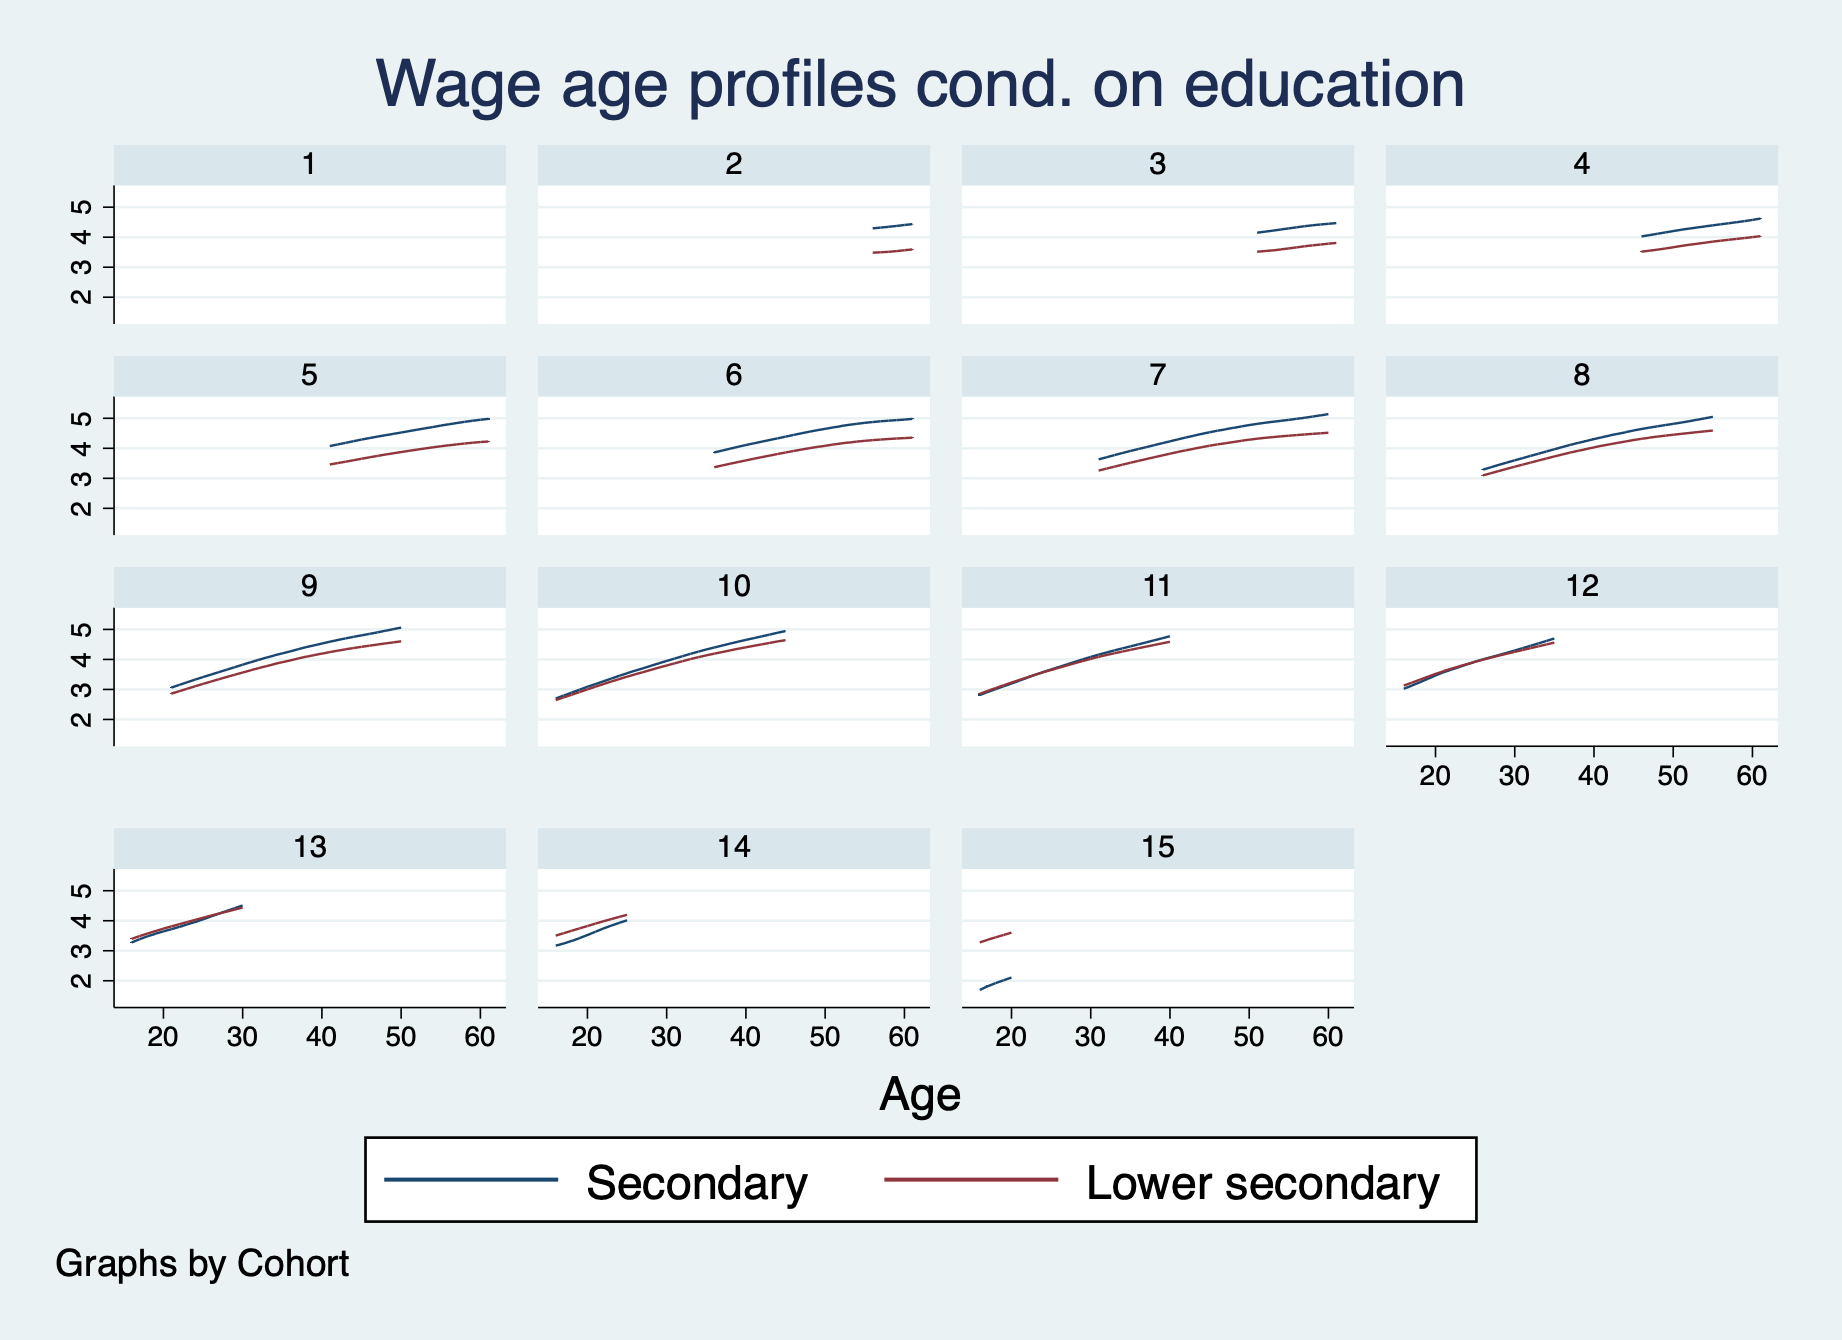
\includegraphics[scale=0.4]{graph1.png}
    \caption{\label{fig:pred_reg}Predicted wage-age profiles by cohort}
    
\end{figure}
\begin{figure}
    \centering
    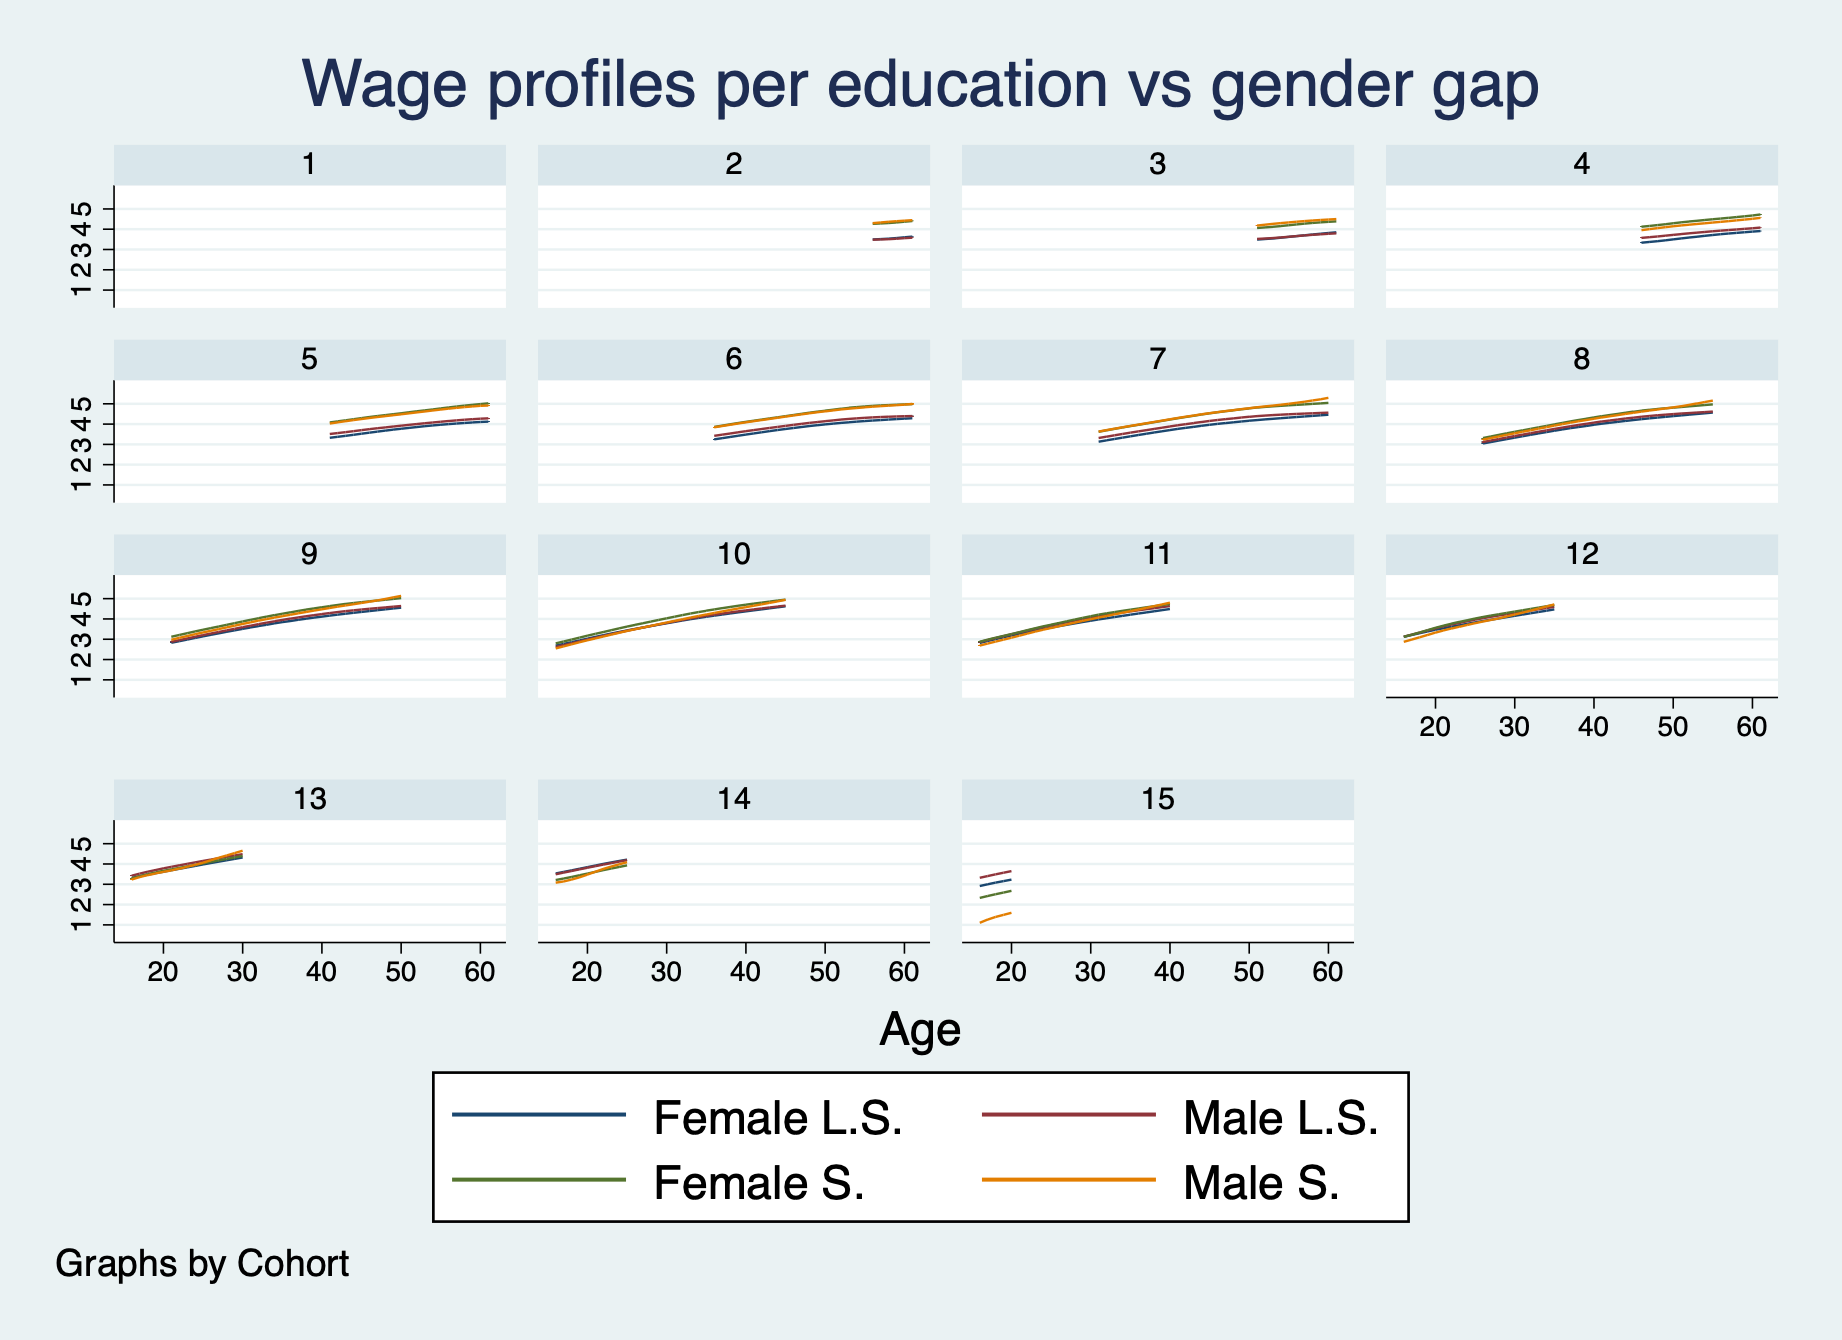
\includegraphics[scale=0.4]{graph2.png}
    \caption{\label{fig:w_gend_l}Gender gap in the wage age profiles for different education level}
    
\end{figure}

\begin{figure}
    \centering
    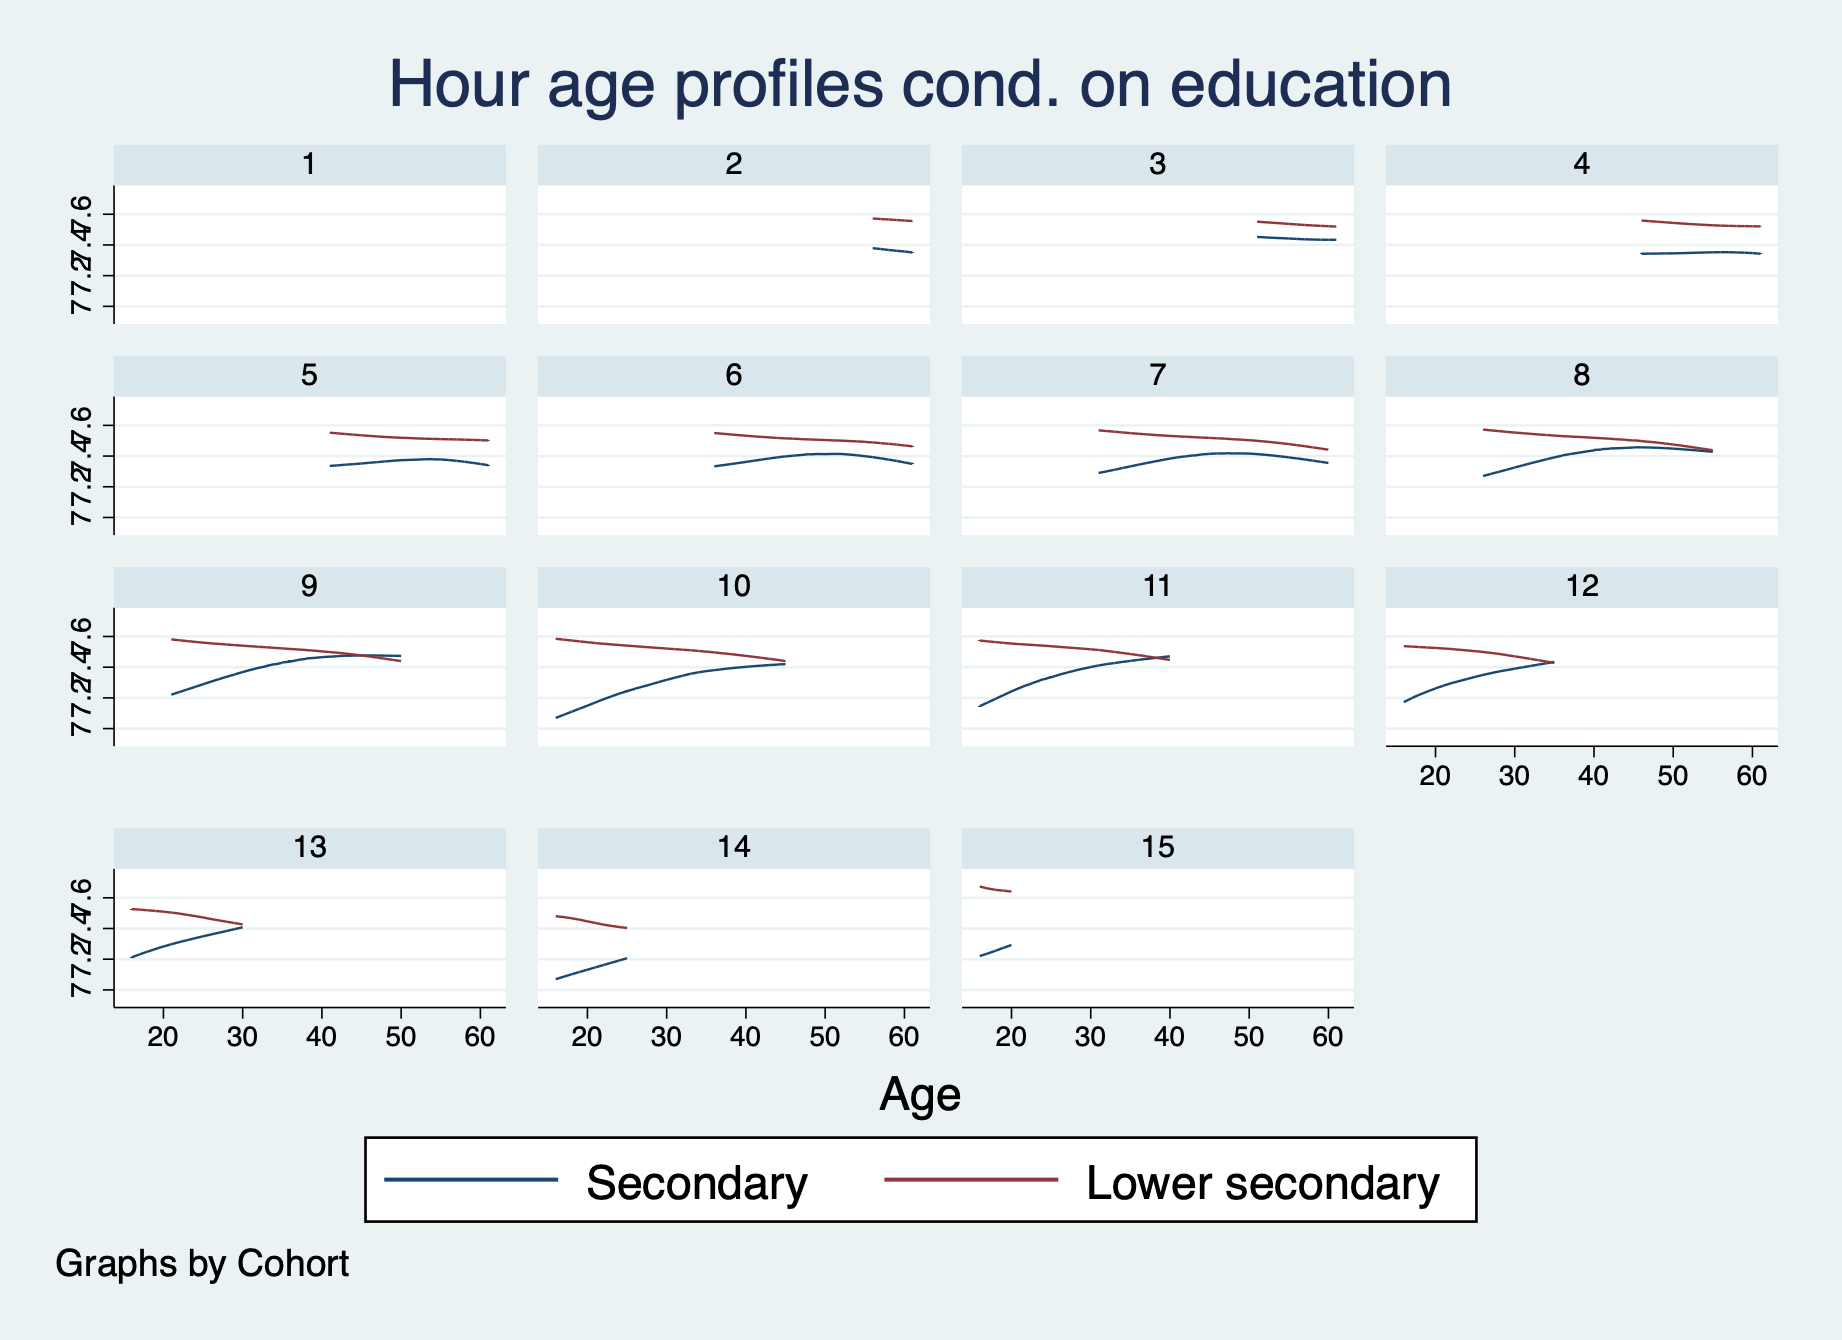
\includegraphics[scale=0.4]{graph4.png}
    \caption{\label{fig:hours}Hours-age profile}
    
\end{figure}
\begin{figure}
    \centering
    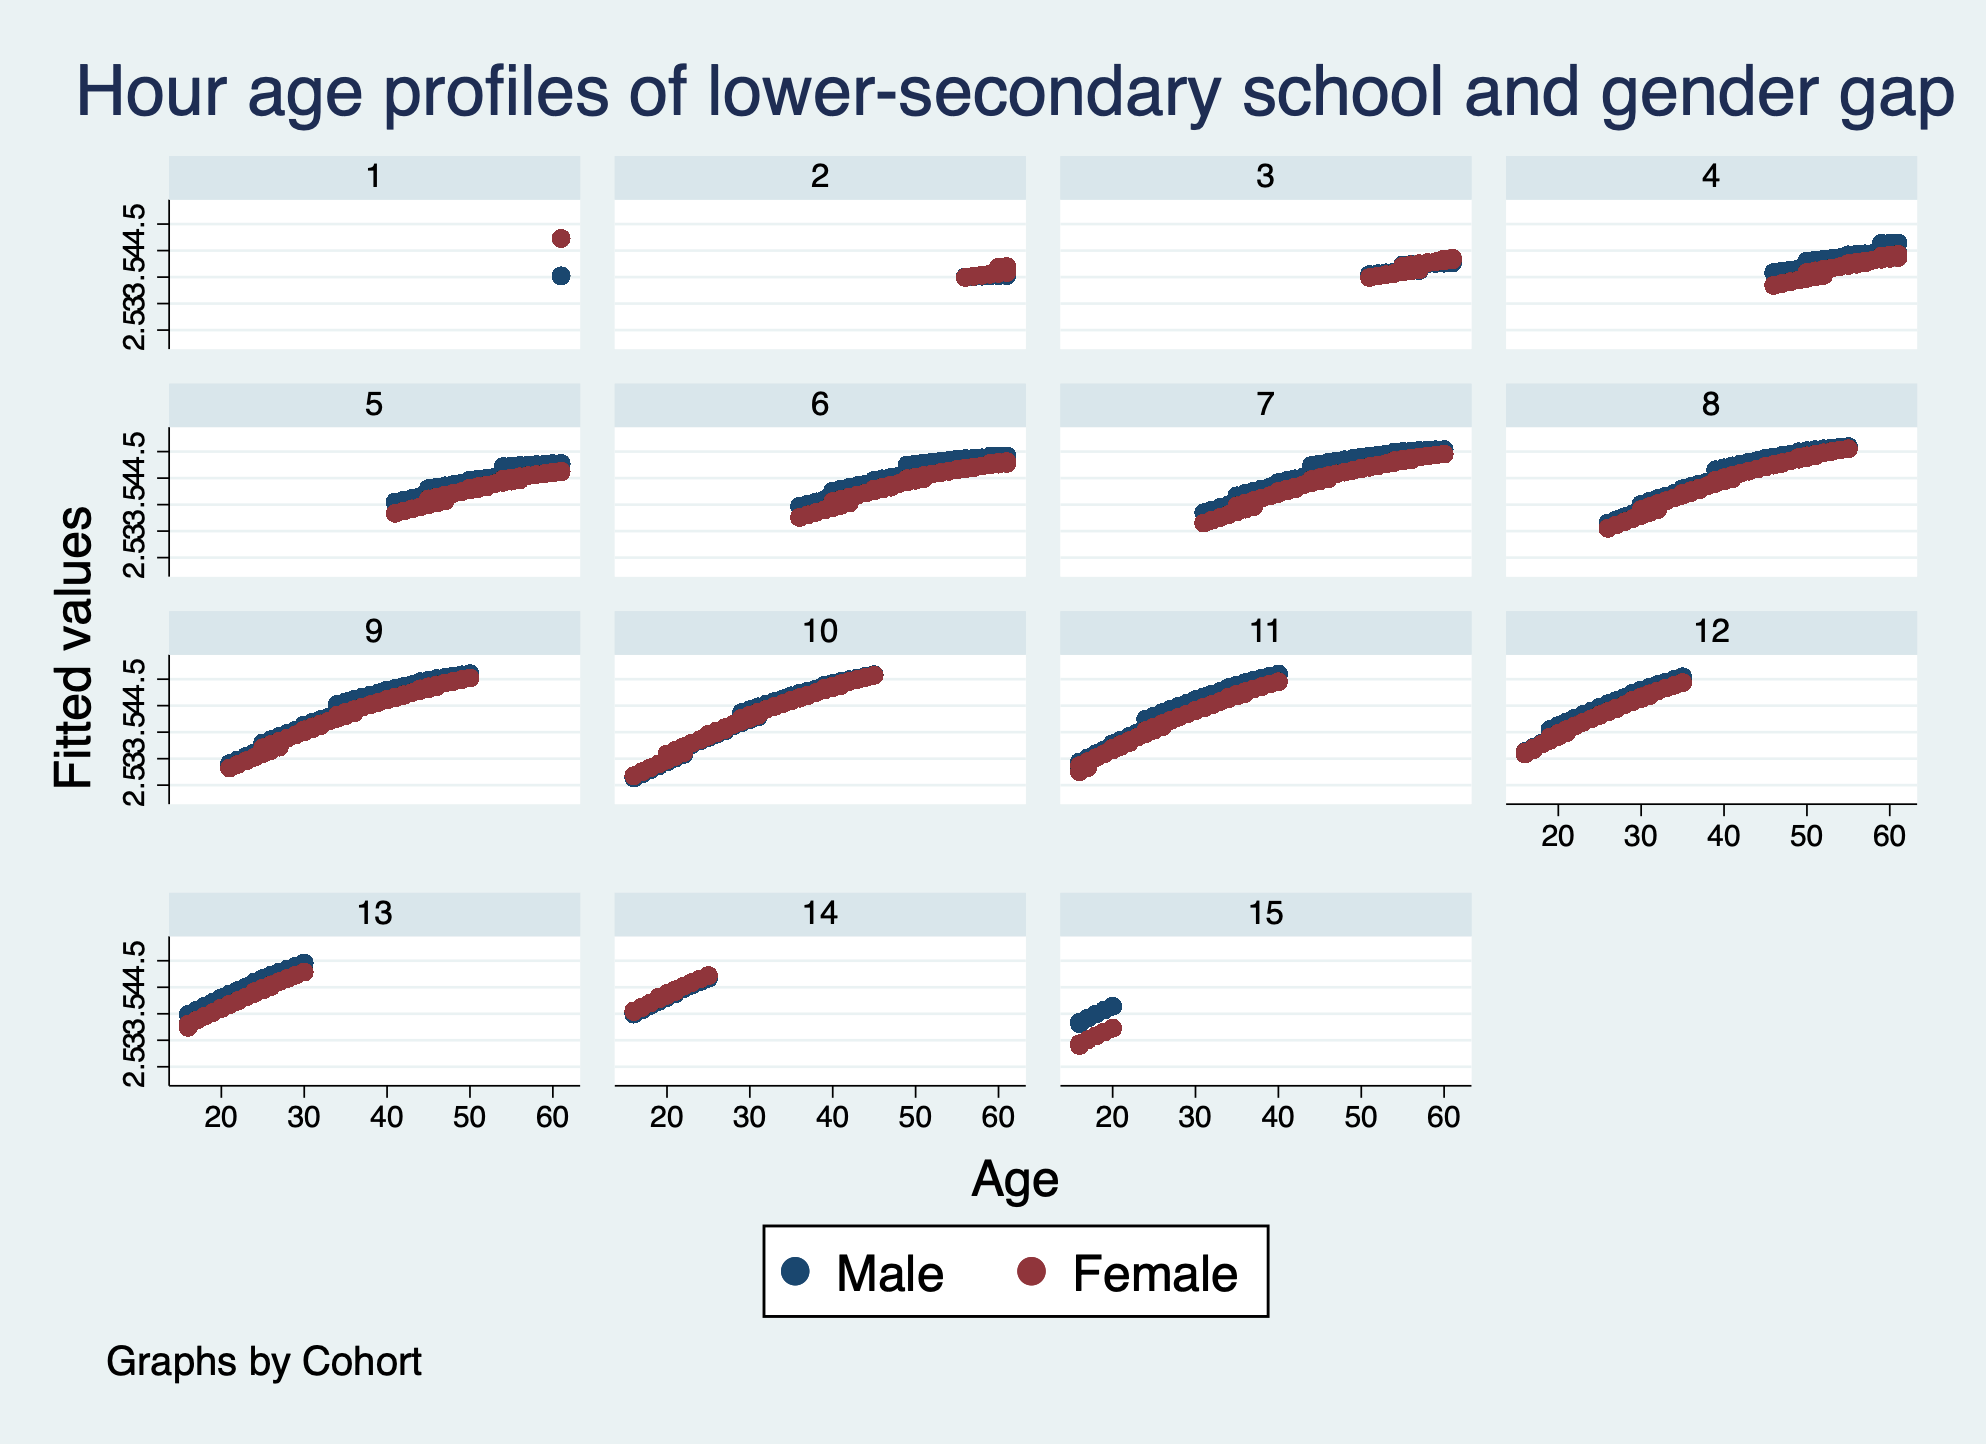
\includegraphics[scale=0.4]{graph5.png}
    \caption{\label{fig:h_l_cohorts}Hours-age profile and gender gap}
\end{figure}

\end{document}


